\documentclass{beamer}

\usefonttheme{serif}
\usepackage{charter}

\usepackage[utf8]{inputenc}
\usepackage[english]{babel}
\usepackage{listings}
\usepackage{graphicx}
\usepackage{epstopdf}

\setbeamertemplate{navigation symbols}{}
\setbeamertemplate{footline}[frame number]{}
% \setbeamertemplate{footline}{\hfill\insertframenumber~\vrule~\inserttotalframenumber}
\lstset{
  stepnumber=1,
  breaklines=true,
  basicstyle=\ttfamily\scriptsize,
  numberstyle=\tiny,
  commentstyle=\color{gray},
  showstringspaces=false,
  keepspaces=true,
  escapeinside=\#\#
}

\renewcommand\big[1]{
  \begin{center}
    \Large{#1}
  \end{center}
}

\begin{document}

\begin{frame}
  \centering\Huge{GNU Parallel}
\end{frame}

\begin{frame}
  \big{This is fucking pathetic}
  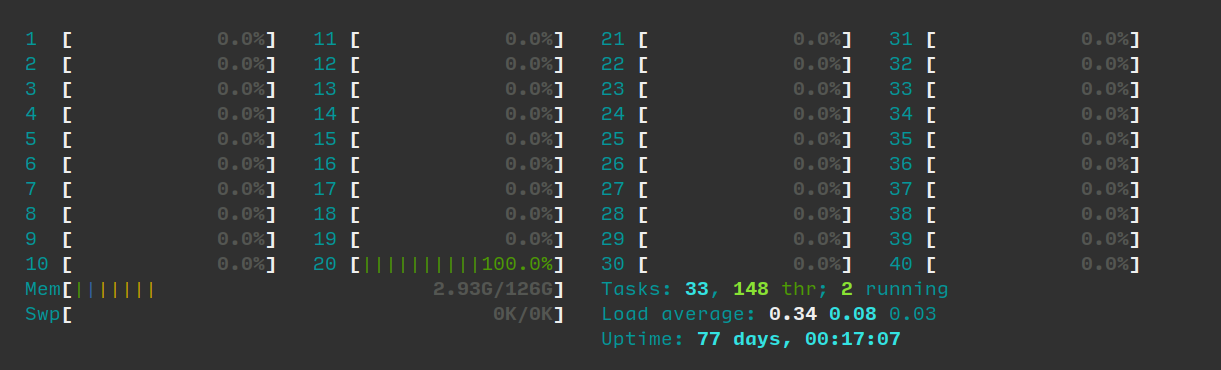
\includegraphics[scale=0.25]{pathetic.png}
\end{frame}

\begin{frame}
  \big{This is fucking awesome}
  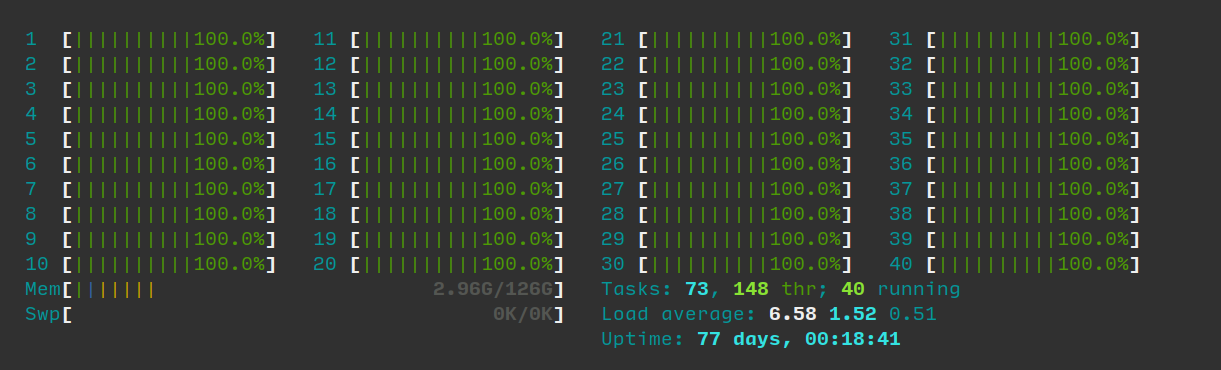
\includegraphics[scale=0.25]{awesome.png}
\end{frame}

\begin{frame}
  \big{Parallel can transform pathetic into awesome\ldots}
  \pause
  \big{But it sucks.}
  \pause
  \begin{itemize}
    \item \textbf{Its user interface is weird}
    \item It pesters you for credit and money
    \item It can make some jobs \emph{slower}
    \item It's written in Perl
  \end{itemize}
\end{frame}

\begin{frame}[fragile]
  \big{The Extortion Scheme}
  \tiny
\begin{verbatim}
~ :) parallel echo ::: 1 2 3
Academic tradition requires you to cite works you base your article on.
When using programs that use GNU Parallel to process data for publication
please cite:

  O. Tange (2011): GNU Parallel - The Command-Line Power Tool,
  ;login: The USENIX Magazine, February 2011:42-47.

This helps funding further development; AND IT WON'T COST YOU A CENT.
If you pay 10000 EUR you should feel free to use GNU Parallel without citing.

To silence this citation notice: run 'parallel --citation'.
\end{verbatim}
\end{frame}

\begin{frame}[fragile]
  \big{``Shut up, parallel!''}
\begin{verbatim}
~ :) parallel --citation

[...]

Type: 'will cite' and press enter.
> will cite

Thank you for your support. It is much appreciated.
The citation notice is now silenced.
\end{verbatim}
\end{frame}

\begin{frame}
  \big{The mental model}

  Use \texttt{parallel}'s template language and operators to build a list of commands to run.
\end{frame}

\begin{frame}[fragile]
  \big{::: and \{\}}
  \begin{description}
    \item[:::] Pass command-line args to template.
    \item[\{\}] Replace with each item in the list.
  \end{description}

\begin{verbatim}
~ :) parallel {} ::: date uname 'uptime -s'
Tue Oct 22 13:54:53 EDT 2019
Linux
2019-09-30 13:06:13

~ :) parallel 'du -h {}' ::: *.txt
4.0K  chars.txt
4.0K  demenage.txt
16K   UTF-8-demo.txt
\end{verbatim}
\end{frame}

\begin{frame}[fragile]
  \big{Mulitple invocations of :::}
  Creates a permutation of the elements
\begin{verbatim}
~ :) parallel 'echo {}' ::: a b ::: 1 2 ::: x y
a 1 x
a 1 y
a 2 x
a 2 y
b 1 x
b 1 y
b 2 x
b 2 y
\end{verbatim}
\end{frame}

\begin{frame}[fragile]
  \big{:::+}
  Similar to ::: but works pair-wise
\begin{verbatim}
~ :) parallel 'echo {}' ::: a b :::+ 1 2 :::+ x y
a 1 x
b 2 y
\end{verbatim}
\end{frame}

\begin{frame}[fragile]
  \big{::: and :::+}
  The operators ::: and :::+ can be mixed and matched
\begin{verbatim}
~ :) parallel 'echo {}' ::: a b ::: 1 2 :::+ x y
a 1 x
a 2 y
b 1 x
b 2 y
\end{verbatim}
\end{frame}

\begin{frame}[fragile]
  \big{Positional placeholders}
  The placeholder \texttt{\{n\}} can be used to select the nth element in the list item.
\begin{verbatim}
~ :) parallel 'echo {3} {1} {3}' ::: a b ::: 1 2 :::+ x y
x a x
y a y
x b x
y b y
\end{verbatim}
\end{frame}

\begin{frame}[fragile]
  \big{:::: and ::::+}
  Similar to ::: and :::+, but they take their arguments from files.
\begin{verbatim}
~ :) cat digits.txt
1
2
3
~ :) parallel 'echo {}' :::: digits.txt
1
2
3
\end{verbatim}
\end{frame}

\begin{frame}[fragile]
  \big{stdin can be used as a file}
\begin{verbatim}
~ :) seq 1 3 | parallel 'echo {}' :::: -
1
2
3

~ :) seq 1 3 | parallel 'echo {}'
1
2
3
\end{verbatim}
\end{frame}

\end{document}
